%!BIB TS-program = biber

\documentclass[a4paper,12pt]{article}
\usepackage[utf8]{inputenc}
\usepackage[english]{babel}
\usepackage{graphicx}
\usepackage{float}
\usepackage{comment}

\usepackage[
backend=biber,
style=alphabetic,
sorting=ynt
]{biblatex}

\addbibresource{refy.bib}
\usepackage{geometry}
 \geometry{
 a4paper,
 total={170mm,257mm},
 left=20mm,
 top=20mm,
 }
\usepackage{framed}
\graphicspath{ {./images/} }

\usepackage{hyperref}
\usepackage{amsmath}
\usepackage{amsfonts}
\usepackage{caption}
\captionsetup[figure]{font=small}
\usepackage{listings}


\usepackage{environ}
\usepackage{etoolbox}



\begin{document}

\section{Abstract}

"Might of Timaert" is an indie 2d procedural RPG with tile graphics. Game engine is based on cellular automata with a "real time" (game tick/10 $us$) world simulation. Cellular world is connected 1024x1024 array of cells with torus topology. All the physics (zones, fluids, climate etc.) is simulated on ancilla arrays. All the world objects are dynamically linked to relevant cells. It is expected to subsequently have an order of $10^4$ individual active game objects. Menus, fights, quests and others player-game interactions are realised using finite automata world states.

Games references: $mount-and-blade, dwarf-fortress, caves-of-qud, Elona+, fear-and-hunger$

Contact email:  
\href{mailto:jirnyak@gmail.com}{jirnyak@gmail.com} 
Telegram: 
\href{https://t.me/mankobus}{\nolinkurl{@mankobus}}
 GitHub: 
\href{https://github.com/Jirnyak}{\nolinkurl{Jirnyak}}

\begin{figure}[H]
    \centering
    
\includegraphics[height=4.5cm]{images/witch.png}
    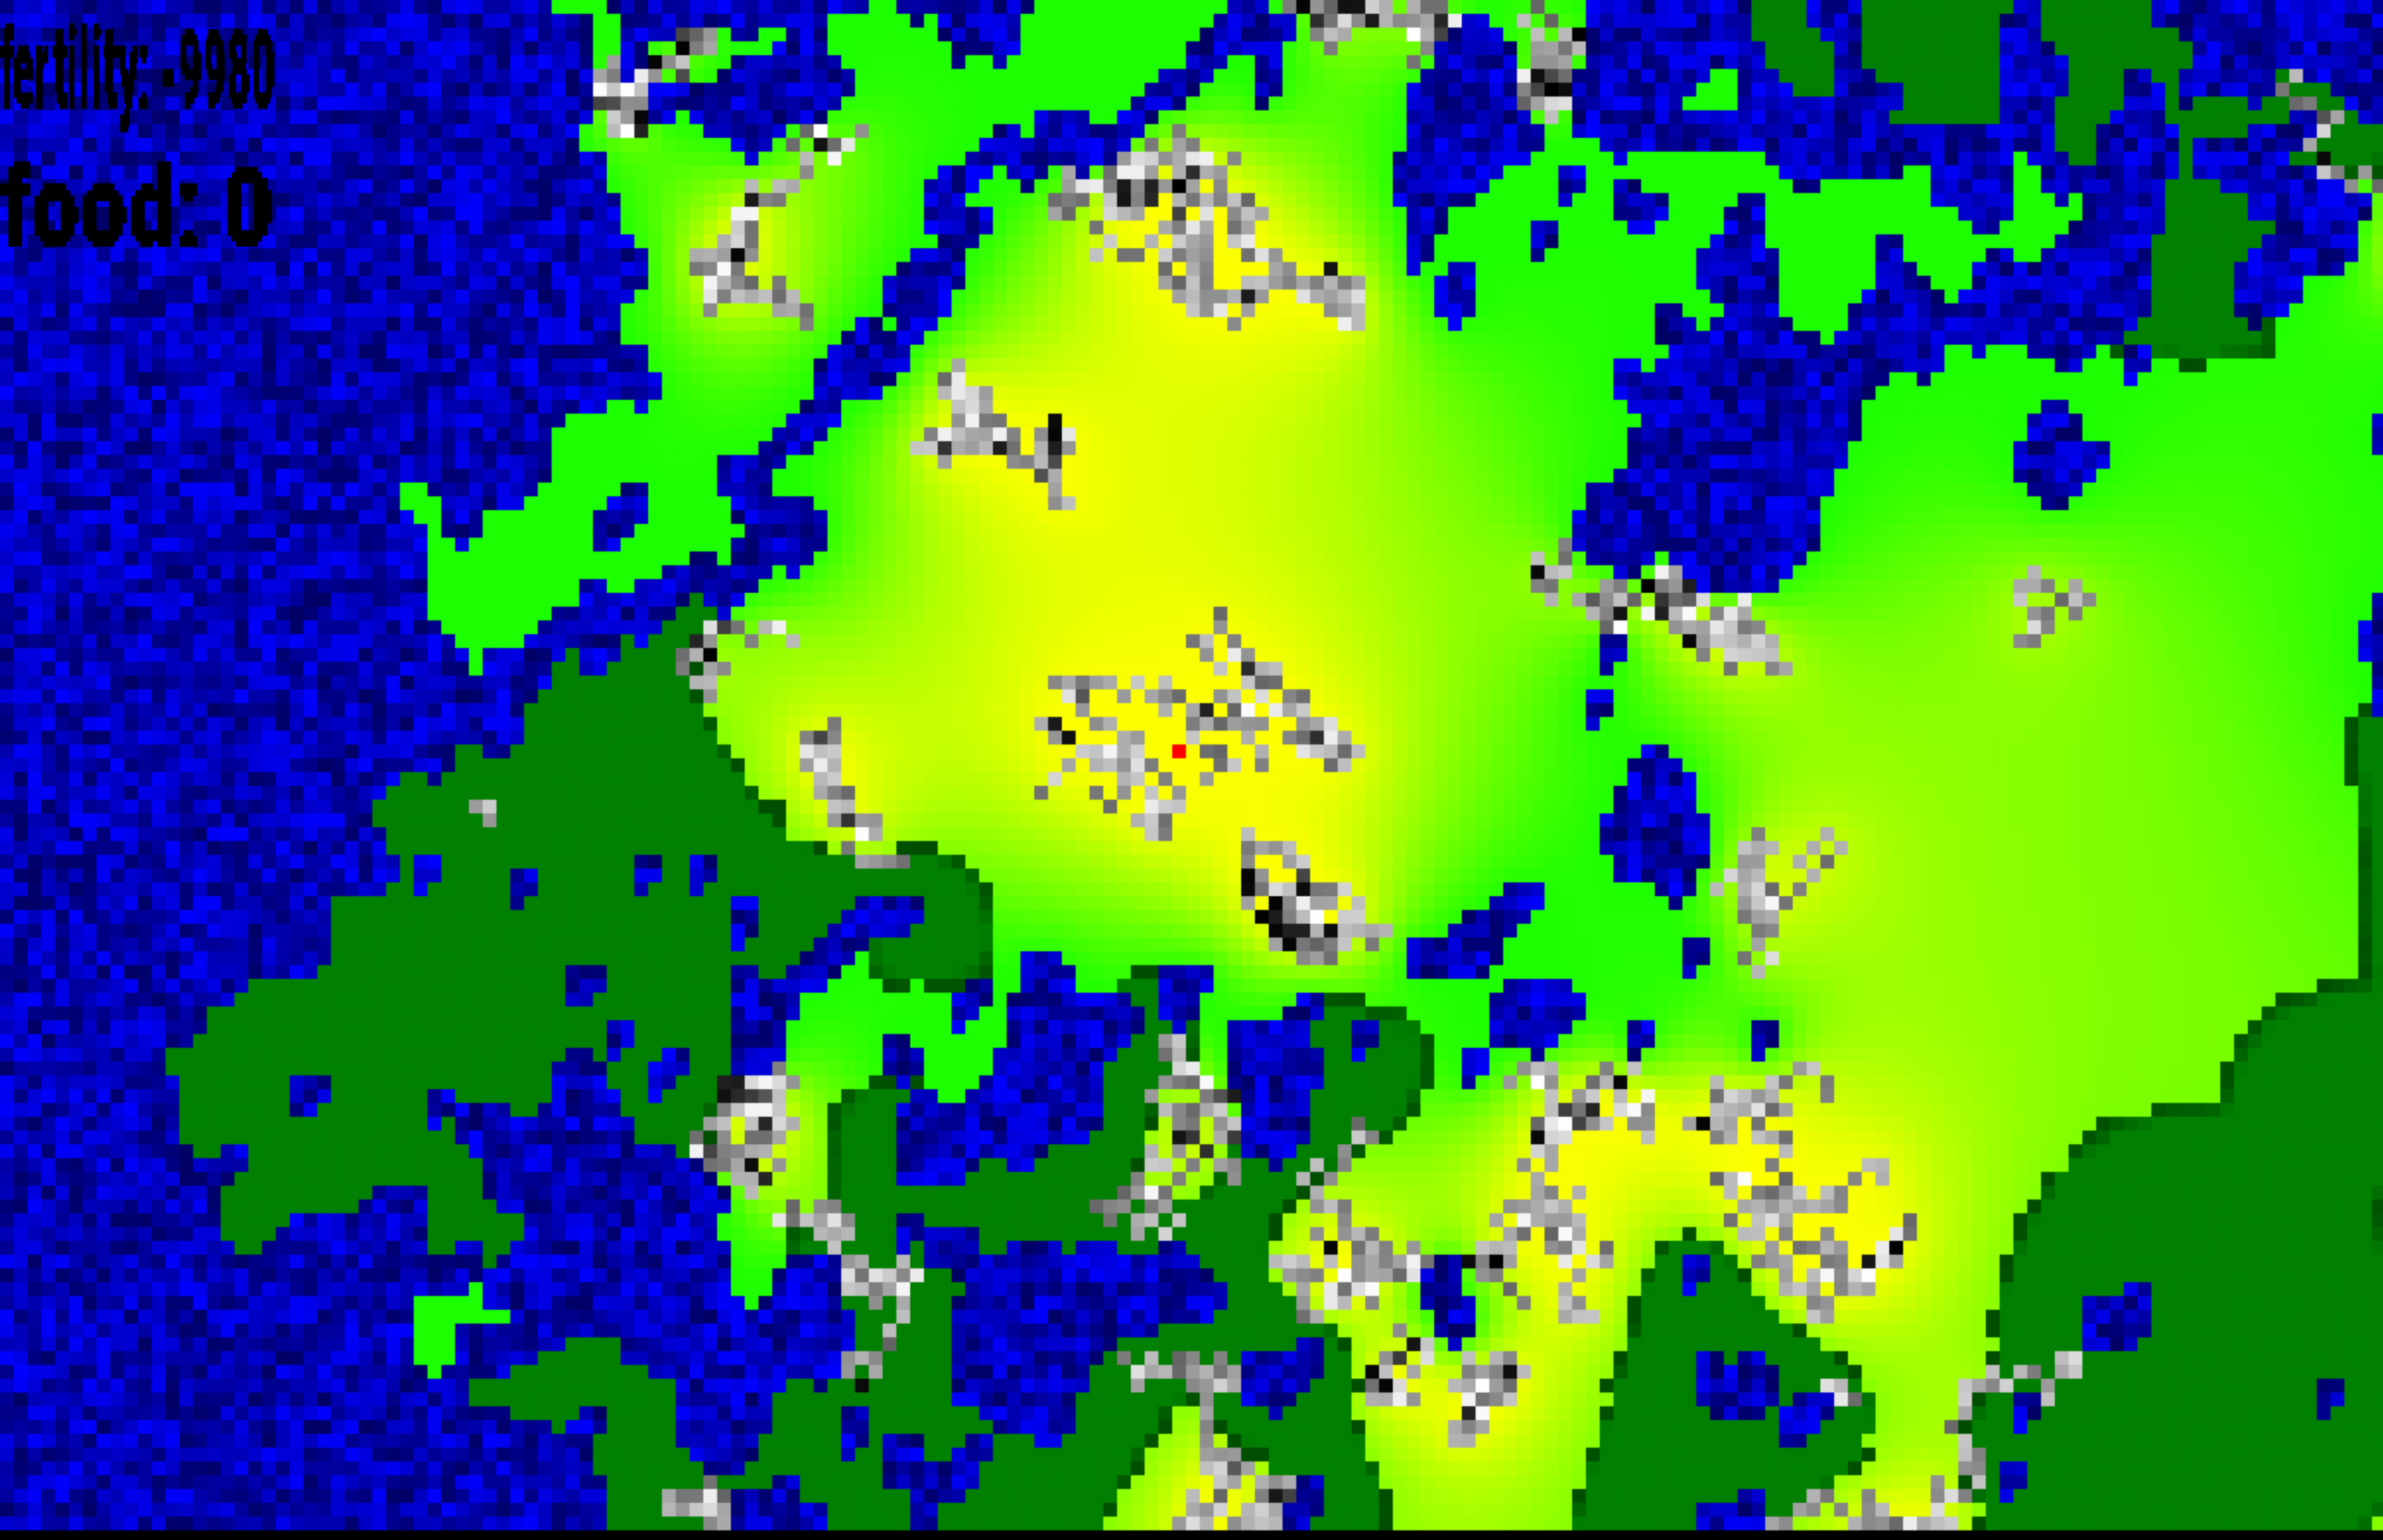
\includegraphics[height=4cm]{images/terrain.png}
    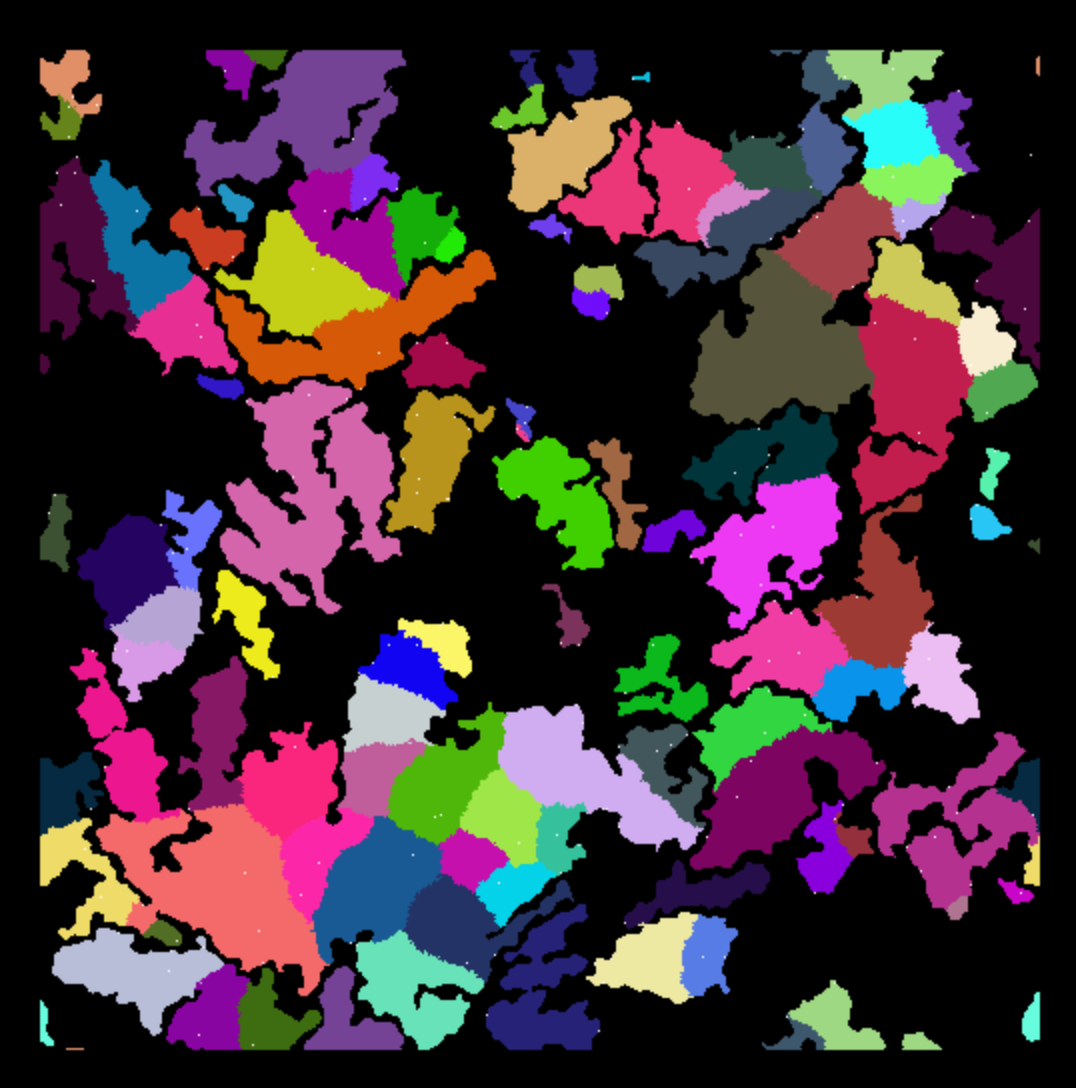
\includegraphics[height=4.5cm]{images/nations.png}
    \caption{1. An example of in game procedural quest.  2. An example of climatic zones. 3. An example of political map. Screenshots from game prototype.}
    \label{fig:witch}
\end{figure}

Download game prototype:
\href{https://drive.google.com/drive/folders/1TWdjQCXN2TFRXHNwMoggdR0XF6cGWThE?usp=sharing}{\nolinkurl{drive.google.com}}


\newpage

\tableofcontents



\newpage

\section{Introduction}

Might of Timaert simulates a large-scale single-player open world game with persistent landmarks and emergent behaviours (similar to Mount & Blade-style campaign world simulation). The design separates the global strategic layer (map, kingdoms, resources, population) from turn-based tactical fights and action, and real-time landmark exploration.

Introduction will cover central game ideas and systems, and the next sections will expand each main system in detail - RPG Mechanics \autoref{sec:RPG}, Economics  \autoref{sec:economics}, Politics, Lore, Events("Quests"), Global World, Local World, Fight Mode, AI, and Gameplay. Also, Spells, Skills, Perks, Monsters and Artefacts lists are attached.

\begin{figure}[H]
    \centering
    \includegraphics[height=8 cm]{images/test.png}
    \caption{A test image.}
    \label{fig:example}
\end{figure}

\begin{equation}
    E = mc^2
    \label{eq:example}
\end{equation}

\newpage

\subsection{Core Concepts}

\subsubsection{Global World:} is a 1024x1024 cells toroidal manifold. Most game is spent in a global regime where player, NPCs and different creatures (peasants, caravans, bandits, demons, pilgrims, armies) are travelling between cities and landmarks or gathering resources. It is a connected world map where nature (forests, climate, resources), economics (cities, villages, caravans) and politics (kingdoms, armies, wars) are simulated in real time. Time passes in hours in the Global World. Seed is used to generate the  Global World. There could potentially be many different global worlds, which are generated and stored as saved data and accessed when the player enters a specific world. It is expected to take tens of game years for a player in the Global World for an average playthrough. If around 60 FPS, one IRL second will be one hour of game time. The game could be paused in the Global World at any time, but real time linear flow of game ticks simulation if not. One year is 365 in-game days, so it will take around 20 hours of real-time gameplay for an average 10 years walkthrough, but the game speed could be increased. 

References: mount and blade, civilization, crusader kings.

\subsubsection{Cell} 

The smallest unit of the strategic global world grid. Contains position data and holds objects, terrain type, resources arrays, faction owner politic map info, and danger zone levels. 2 D cellular connected world is inspired by the Lattices and Ising chains model in physics. Cellular structures are used for many emergent simulations and systems:

\begin{itemize}

\item \textbf{Resources} arrays. Each cell is mapped by a number of any resource deposited inside (usually 0). Resources are divergent and distributed unevenly. Economic.

\item \textbf{Factions} arrays. Each cell is mapped by a number representing the political owner faction. It creates a political map of the world. The owner of the cell owns a Landmark in it and its taxes and resources. Politics.

\item \textbf{Level zone} array. Each cell is mapped by a zone difficulty level number, which changes over game and time evolutions and as a function of landmarks and other systems. For example, there are lower-level zones around cities and higher-level zones around ruins. Also, different parts of the Global World have naturally different difficulties. Zone level affects RPG aspects such as enemies, encounters, ambushes prob, loot quality, and exp coefficients. RPG.

\item Local \textbf{event} threads. Most of the events in the game are local and read only by adjacent coordinates. 

\end{itemize}

\subsubsection{OBJ}  

Any interactive, unique entity in the world: player, NPCs, caravans, armies, spell effects (portals, meteors), or landmarks (villages, cities, ruins). Objects are managed by the ENTT system. Every object has its own parameters, such as name, economy value, and RPG attributes. Each object also has its own inventory array. For example, peasants or caravans carry resources and goods. Cities and Landmarks stock resources and different items. Locan World can place items from the Landmark inventory inside for the player to potentially collect.

\subsubsection{Landmark} 

A persistent, typically non-movable object, such as cities, castles, ruins, or monster dens. Landmarks can change state, be created, or destroyed, but such events are rare. Landmarks are the main anchors of gameplay - RPG, economic, politics and quests hubs. A player or NPC can create their own Landmark if the specific conditions are fulfilled. Here is a list of the most important Landmarks:

\begin{itemize}

\item \textbf{Villages} generated near large resource deposits. Spawn peasant squads who gather resources and supply adjacent cities in exchange for small gold. Provide quests.

\item \textbf{Cities} generated as a centre of mass of a set of villages. Accumulate resources and produce goods, caravans, armies and taxes for the owner faction. Provide many quests.

\item \textbf{Castles} generated on political borders. Spawns armies of the owner faction. Home for powerfull NPC and quests.

\item \textbf{Ruins} generated far from cities and villages. Spawns cultists and hold powerfull procedural black artefacts. Target of quests and dark corruption mechanics - ruins spread corruption, increasing the level of the zone over time.

\end{itemize}

\textbf{Game state}

 A specific game mode gives information to the player (map, stat screen) or allows interactions with the world. A UI style for game state screens are dark, warm beige-reddish palette to give a dark medieval paper-wooden feel.
 
 \begin{itemize}
 
 \item \textbf{Main menu} - the first thing the player sees when running the game. Here player can start a new game, load a saved one, do a detailed world generation setup and exit the game. Later homologous menu could be opened in-game for saving, loading, restarting, and exiting purposes.
 
 \item \textbf{Game screen} - a render of a zoomed-in or out fragment of the Global World. Different interface buttons, such as stat, menu, and interaction buttons. Essential UI such as current player HP, MP, and SP resources. Most other UI and states are popping on top of the Game Screen.
 
  \item \textbf{Character creation} - when starting a new game, a player can choose a name, sex, class (initial skills) and portrait for their new character. Birth options will affect where the player starts geographically (climate zones, near water or mountains, owner territories - Magica, Empire, Timaert, Barbaric). Lore.
 
 \item \textbf{Stat screen} - a UI multibox of all the Player object parameters, including RPG, inventory and politics systems. Here also the player can check and reorganise inventory, spend skill, atrribute and perk points. RPG.

 \item \textbf{Map mode} - a full map render of the Global or Local World map (depedning of where the player is present at the moment). By default, the Map will be obscured from the player by unseen flags on non-visited far cells, to stimulate the player's exploration instinct. Additionally, it also have resources depositions modes and politic map. Resources are also obscured, or their numbers are rounded, but could be shown with greater accuracy if the player has specific skills (prospecting, scouting, etc.) Exploration, Politics and Economics.
 
 \item \textbf{Interaction mode} - universal hub for interobject and player-object interactions when nearby in the Global World. Allows a list of options to Talk, Trade, Quest, Fight, and Leave states calls. Intercation mode is also simulated as a finite automata state model for object-object interactions during the simulations - for example, bandits extorting money from peasants or plot-driven NPC interactions during the Global World simulation. A pair of particle interaction event as in physics in game space-time.
  
 \item \textbf{Fight mode} - Important part of gameplay, Player object will face symmetrical in terms of RPG mechanics in game object and use tactics, items, spells, and build optimisation to slay the enemy. Uses RPG mechanics. The player can flee from the fight and use many different active spells(skills). Most enemy faction members will initiate fight mode with the player regardless of what options in interaction mode the plyer chosen. If the player has chosen to fight with a neutral object, the owner faction's relation with the player will decrease. Weaker objects will try to flee or buy out. Stronger objects will be more aggressive. Some builds are fight mode oriented, others are more economy and political or exploration focused (this comes from RPG attributes and skills distributions). Usually, fighting is the main source of EXP and LOOT. Fight mode is also simulated for object-object interactions behind the scenes during the Global World simulation. RPG.
 
 \item \textbf{Trade mode} - Inventory exchange mode. Where the player and object or landmark or object-object could barter any items from their inventories. It depends on RPG and economics, and also each in-game item, such as resources, goods, gold or arms, has an absolute value parameter which guides pricing together with the economics system. Economics.
 
 \item \textbf{Landmark mode} - while the player is in a landmark cell shows information about the landmark, for example, city owner faction flag, city map, population, quests, etc. The player can also visit Landmark and any other cell, but usually the Local World of Landmark will be of special interest. Anchors. 
 
 \item \textbf{Local mode} - A procedurally or precreated real-time action 2d area of size 1024x1024. It is used for exploration (dungeon maps, labyrinths), quests (find a specific person in a city, find artifact in a labyrinth) and decorative purposes (city population is roaming on the streets). EXP gains are reduced to minimal or non-existent in a Local World. Game time is frozen for balance and immersion purposes. Used for quests. Seed is used to generate Local World, and it is usually generated dynamically from Global World parameters (the city map is generated from a Landmark population).
 subgame with action real-time movement on a gridless space in order to explore, pixel hunt for quests (for example, char sprites of specific features), artefacts, and fun genocide of the local population, which is, of course, punishable by Global fight with guards. A player can walk around living city streets with thousands of living sprites, explore a labyrinth or build their own base in the wilderness (will store local map data on players pc).  Fun and decoration.
 
 \item \textbf{Event mode} - a pop-up of original non-repeating random event, procedural event from local game variables (zone level, objects, economics, politics, etc.) or game state. Usually contains text messages for lore and plot, and sometimes choice option buttons which will affect the outcome and any in-game variables (for example, player stats). Quests.
 
 \item  \textbf{Event log} - A list of all event history with in-game date when it happened to the player for both information and immersion purposes. Journal.
 
 \end{itemize}
 
\subsubsection{Factions}

The world can contain max 128 distinct factions, including lore factions:

\begin{itemize}
\item Shattered Magica Kigdoms - Old Magica, Northern Magica, Southern Magica, Central Magica. North West.
\item Huge centralised - Empire of Light. Equator.
\item Small feudal - Barbaric Kingmods. North East.
\item Trade Republic of Timaert. South or behind the sea.
\item Dark Cults (minor factions)
\item Bandits (minor factions)
\item Wilderness (minor factions) 
\item Uprised Peasants (minor factions)
\item Witches (Demiurgs) (Plot factions)
\item Potentially - Player-owned created faction.
\end{itemize}

Each kingdom has variables:

\begin{itemize}
\item Name, flag.
\item Occupies contiguous territories on the political map.
\item has its own gold capital collected from owned landmark taxation.
\item Spawns units (armies, agents, bosses npcs).
\item Has diplomatic relations with all other factions, $[-127, +127]$ Alliance from + 100 (fight common wars), Trade from + 50 (send caravans), Neutral around 0, Aggression -50 (border confilcts), Total War -100 (send occupation armies).
\item Total population.
\item Key NPCs Leaders (lords).
\item Own Landmarks.

\end{itemize}


\subsubsection{Difficulty Zones}

Zone difficulty increases gradually over long-term game time (years) to preserve progression pressure.

Higher-level landmarks and corrupted territories influence nearby cell difficulty values.

Plot events can significantly change zone difficulties in specific areas.

\subsection{Game Time}

\begin{itemize}
\item Primary simulation tick: 1 in-game minute.
\item 365 days per in-game year.
\item Entities age annually. Human NPCs and even players could die at old age if significant time has passed (chance to die after age > 60).
\item Landmark population updates once per year
\end{itemize}

Movement speed is object RPG stats dependent and the movement in Global Mode consumes SP basing on cell terrain weight.
The average traversal time of one global tile is approximately one in-game day, though fast units may cross in one hour.
Population growth in cities and villages follows a logistic-style model \autoref{eq:sigmoid}:

\begin{equation}
P_{t+1} = P_t + rP_t \left(1 - \frac{P_t}{K} \right)
 \label{eq:sigmoid}
\end{equation}

where $r$ is the growth coefficient and $K$ is the carrying capacity (around one million pop cap).









\newpage

\section{RPG Mechanics}
\label{sec:RPG}

A performance-first RPG architecture designed to be universal for all entities (players, NPCs, enemies).

Character progression is driven by:

\begin{itemize}
\item Classes — determine starting skills; additional skills learned during playthrough
\item Levels — grant attribute points, skill points and perk points.
\item Fame — political and economic power (owned territories, capital, deeds)
\end{itemize}

The system is structured into five core layers:

\begin{enumerate}
\item Attributes — percentage multipliers and event check determinants
\item Skills — flat base bonuses and tactical unlocks
\item Spells — magic abilities and effects
\item Items — weapons and artifacts with bonuses
\item Perks — strong specialization modifiers
\end{enumerate}

\subsection{Resources}

\begin{table}[H]
\centering
\begin{tabular}{|c|c|c|}
\hline
Resource & Purpose & Critical State \\
\hline
HP & Health & $\leq 0 \rightarrow$ Dead \\
MP & Spell casting & Cannot cast if empty \\
SP & Actions / Movement & $\leq 0 \rightarrow$ HP damage \\
\hline
\end{tabular}
\end{table}

Primary governing attributes:

\begin{itemize}
\item HP $\rightarrow$ END
\item MP $\rightarrow$ WIL
\item SP $\rightarrow$ SPD
\end{itemize}



\subsection{Attributes}

Nine primary attributes:

\begin{table}[H]
\centering
\begin{tabular}{|c|c|}
\hline
Attribute & Effect \\
\hline
STR & +1\% physical damage; carry weight \\
END & +1\% HP regen; increases HP \\
AGI & +1\% SP regen; dodge \\
WIL & +1\% MP regen; increases MP \\
INT & +1\% spell damage; +1 active spell slot per point \\
WIS & +1\% EXP gain; +1 learned spell slot per point \\
LCK & Improved loot; crit chance \\
CHA & +1 relation; −1\% trade tariffs \\
SPD & Movement speed scaling (asymptotic); increases SP \\
\hline
\end{tabular}
\end{table}

\subsection{Level and Experience System}

Level data:

\begin{itemize}
\item $level$
\item $exp$
\item $exp\_to\_next$
\item $skill\_points$
\end{itemize}

\subsubsection{Level Rewards}

Per level:

\begin{itemize}
\item +3 Skill Points
\item +3 Attribute Points
\item +1 Perk Point every 10 levels
\end{itemize}

Starting at level 1:

\begin{itemize}
\item 9 Attribute Points
\item 5 Skill Points
\item 1 Perk Point
\item 3 Class skills
\end{itemize}

\subsubsection{Experience Formulas}

\begin{equation}
EXP_{next}(lvl) = 1000 \cdot lvl \cdot (0.1 \cdot lvl + 1)
\end{equation}

\begin{equation}
EXP_{fight}(lvl_m, k) = 10 \cdot lvl_m \cdot k
\end{equation}

\begin{equation}
EXP_{quest}(lvl_q, k) = 100 \cdot lvl_q \cdot k
\end{equation}

Where:

\begin{itemize}
\item $k$ — difficulty modifier
\item $lvl_m$ — monster level
\item $lvl_q$ — quest level
\end{itemize}



\subsection{Combat Stats}

\subsubsection{Hit Points}

\begin{equation}
HP(HP_0, END) = HP_0 \cdot (1 + 0.1 \cdot END)
\end{equation}

Base HP: 100

\subsubsection{Mana Points}

\begin{equation}
MP(MP_0, WIL) = MP_0 \cdot (1 + 0.1 \cdot WIL)
\end{equation}

Base MP: 10

\subsubsection{Stamina Points}

\begin{equation}
SP(SP_0, SPD) = SP_0 \cdot (1 + 0.1 \cdot SPD)
\end{equation}

Base SP: 100



\subsubsection{Regeneration}

\begin{equation}
HP_{regen} = base\_hp\_regen \cdot (1 + 0.1 \cdot END)
\end{equation}

\begin{equation}
MP_{regen} = base\_mp\_regen \cdot (1 + 0.1 \cdot WIL)
\end{equation}

\begin{equation}
SP_{regen} = base\_sp\_regen \cdot (1 + 0.1 \cdot AGI)
\end{equation}



\subsection{Derived Bonuses}

\begin{align}
phys\_damage\_mult &= 1 + 0.01 \cdot STR \\
spell\_damage\_mult &= 1 + 0.01 \cdot INT \\
hp\_regen\_mult &= 1 + 0.01 \cdot END \\
mp\_regen\_mult &= 1 + 0.01 \cdot WIL \\
sp\_regen\_mult &= 1 + 0.01 \cdot AGI \\
exp\_mult &= 1 + 0.01 \cdot WIS \\
move\_speed\_mult &= 1 + \frac{SPD}{SPD + 50} \\
trade\_discount &= 0.01 \cdot CHA \\
relation\_bonus &= CHA
\end{align}



\subsection{Combat Probabilities}

Dodge:

\begin{equation}
dodge = \frac{AGI_{def}}{AGI_{def} + AGI_{att} + K}
\end{equation}

Critical hit:

\begin{equation}
crit = \frac{LCK_{att}}{LCK_{att} + LCK_{def} + K}
\end{equation}



\subsection{Skills}

Skills:

\begin{itemize}
\item Provide flat base bonuses
\item Do not modify attributes
\item Do not apply percentage multipliers
\item Scale linearly
\end{itemize}

Final stat calculation order:

\begin{equation}
FinalStat =
(Base + \sum SkillBase + \sum ItemBase)
\times AttributeMultipliers
\times SituationalMultipliers
\end{equation}

\subsection{Example Skills}

\subsubsection{Bodybuilding}

\begin{equation}
BaseHP = BaseHP_0 + Bodybuilding
\end{equation}

\subsubsection{Swordsman}

\begin{equation}
BaseWeaponDamage = BaseWeaponDamage_0 + Swordsman
\end{equation}

\begin{equation}
BaseSP_{cost} = BaseSP_{0} \cdot (1 - 0.005 \cdot Swordsman)
\end{equation}

Certain skills and spells affect both Global and Tactical layers.

Examples:

\begin{itemize}
\item Scouting increases map visibility (scout vision, scavenge resources).
\item Strategic spells may alter the landmark state or cell types (armageddon).
\item Tracking (show obj suqads tracks - tracks map array over cells)
\end{itemize}


\subsection{Spells}

Spells consume mana and could be generalised as "active skills".
Spell damage scales with mana invested.

Example: Fireball

\begin{itemize}
\item Base: 10 damage for 10 mana
\item Each additional 10 mana increases base damage by +10
\end{itemize}

This allows flexible scaling depending on build and resource availability.


\subsubsection{Travel}

\begin{equation}
BaseSP_{cost} = BaseSP_{0} \cdot (1 - 0.01 \cdot Travel)
\end{equation}


\subsection{Perks}

\begin{itemize}
\item Strong and build-defining
\item Contain advantage and a disadvantage
\item Permanent choice
\item 1 perk at level 1
\item +1 every 10 levels
\end{itemize}

Full perk list is provided in \autoref{sec:perks}.









\newpage

\section{Economics}
\label{sec:economics}

A performance-first economic simulation for a fantasy RPG world, designed to be \textbf{universal for all settlements and factions}. The system is modular, extensible, and supports emergent trade, local markets, and dynamic political control.



\subsection{Core Components}

\subsubsection{World Grid}

\begin{table}[H]
\centering
\begin{tabular}{|c|c|}
\hline
Property & Description \\
\hline
Size & 1024 $\times$ 1024 cells \\
Cell Properties & terrain, resources, cost \\
Resource Fields & Modular, see below \\
\hline
\end{tabular}
\end{table}



\paragraph{Resource Fields}

Each cell:

\begin{equation}
R_{cell} = \{ r_1, r_2, ..., r_n \}
\end{equation}

Each resource:

\begin{equation}
r_i = (type, amount)
\end{equation}

\begin{table}[H]
\centering
\begin{tabular}{|c|c|}
\hline
Resource & Notes \\
\hline
Iron &  \\
Fertility & Crop potential \\
Clay &  \\
Wood & trees \\
Gold &  \\
Water &  \\
Coal &  \\
Gems &  \\
Fur &  \\
\hline
\end{tabular}
\end{table}



\subsection{Landmarks}

\begin{table}[H]
\centering
\begin{tabular}{|c|c|}
\hline
Type & Description \\
\hline
Village & Resource gathering, local trade \\
City & Production, trade, politics \\
\hline
\end{tabular}
\end{table}

Each landmark:

\begin{equation}
L = (population, inventory, location, production\_capacity)
\end{equation}



\subsection{Population System}

Population drives:

\begin{itemize}
\item Unit spawn rate
\item Production/consumption
\item Caravan count
\end{itemize}



\subsubsection{Population Growth (Logistic)}

\begin{equation}
P_{t+1} = P_t + r \cdot P_t 
\left(1 - \frac{P_t}{K}\right) \cdot F \cdot S
\end{equation}

\begin{table}[H]
\centering
\begin{tabular}{|c|c|}
\hline
Symbol & Meaning \\
\hline
$P_t$ & Current population \\
$r$ & Growth rate (e.g. 0.01) \\
$K$ & Carrying capacity (1M) \\
$F$ & Food sufficiency $0-1$ \\
$S$ & Stability $0-1$ \\
\hline
\end{tabular}
\end{table}

If $F$ or $S$ is low, growth slows or reverses.



\subsubsection{Spawn \& Production}

\begin{table}[H]
\centering
\begin{tabular}{|c|c|}
\hline
Output & Formula \\
\hline
Peasants & $k_p \cdot Population$ \\
Caravans & $k_c \cdot Population$ \\
Production & $k_{prod} \cdot Population$ \\
Consumption & $k_{cons} \cdot Population$ \\
\hline
\end{tabular}
\end{table}

Initial balance:

\begin{equation}
k_{cons} \approx \frac{1}{10} k_{prod}
\end{equation}



\subsection{Villages}

\begin{table}[H]
\centering
\begin{tabular}{|c|c|}
\hline
Function & Description \\
\hline
Gather resources & Peasant squads assigned \\
Store inventory & Local storage \\
Sell/deliver & To caravans/cities \\
\hline
\end{tabular}
\end{table}

\paragraph{Extraction per tick}

\begin{equation}
Extracted = BaseGatherRate \cdot SkillCoef \cdot CellDensity
\end{equation}



\subsection{Cities}

\begin{table}[H]
\centering
\begin{tabular}{|c|c|}
\hline
Function & Description \\
\hline
Buy resources & From villages/caravans/peasants \\
Produce goods & See production chains \\
Spawn caravans & For trade \\
\hline
\end{tabular}
\end{table}

City specialization — labor allocation production percentage of population.



\subsubsection{Taxation \& Politics}

\begin{table}[H]
\centering
\begin{tabular}{|c|c|}
\hline
Concept & Formula / Description \\
\hline
City gold & $Gold_{city} = \alpha \cdot Population + \beta \cdot TradeVolume$ \\
Tax paid & $Gold_{tax} = Gold_{city} \cdot TaxPercentage$ \\
Faction income & $Gold_{faction} = \sum_{i \in cities} Gold_{tax,i}$ \\
Ownership & Each cell/landmark: owner\_faction \\
\hline
\end{tabular}
\end{table}

Faction gold can be used for diplomacy, armies, development, etc.



\subsubsection{Production Chains}

\begin{equation}
k_1 \cdot Resource_A + k_2 \cdot Resource_B 
\rightarrow 
k_3 \cdot Good_C
\end{equation}

\begin{table}[H]
\centering
\begin{tabular}{|c|c|}
\hline
Example & Formula / Notes \\
\hline
Iron + Coal $\rightarrow$ Tools &  \\
Fertility + Water $\rightarrow$ Bread &  \\
Fur + Cloth $\rightarrow$ Clothes &  \\
Clay + Coal $\rightarrow$ Pottery &  \\
\hline
\end{tabular}
\end{table}

Production per tick:

\begin{equation}
Produced = ProductionCapacity \cdot SkillCoef
\end{equation}



\subsection{Inventory Model}

Each landmark:

\begin{equation}
Inventory = \{ item_i : quantity \}
\end{equation}

No global market. All trade is local and emergent.



\subsection{Caravan System}

\begin{table}[H]
\centering
\begin{tabular}{|c|c|}
\hline
Step & Description \\
\hline
1 & Spawn at city \\
2 & Load surplus: $Load_i = \max(Inventory_i - LocalNeed_i, 0)$ \\
3 & Choose destination (profit estimate) \\
4 & Travel (pathfinding) \\
5 & Sell if profitable \\
6 & Buy local surplus \\
7 & Return/redirect \\
\hline
\end{tabular}
\end{table}

Emergent global distribution from price, distance, scarcity.

Transport cost for caravan naturally from SP depletion (minimise SP to gold profit).



\subsection{Market System}

Each item:

\begin{equation}
IntrinsicValue_i
\end{equation}



\subsubsection{Local Market Price}

\begin{table}[H]
\centering
\begin{tabular}{|c|c|}
\hline
Symbol & Meaning \\
\hline
$S_i$ & Local supply \\
$D_i$ & Local demand \\
\hline
\end{tabular}
\end{table}

\paragraph{Demand factor}

\[
\boxed{
\begin{aligned}
\text{Pressure}_i &= 
\ln\Bigl(\frac{D_i + \epsilon}{S_i + \epsilon}\Bigr), \\
P^{target}_i &= 
IV_i \cdot \bigl(1 + \alpha \cdot \text{Pressure}_i \bigr), \\
P_{i,t+1} &= 
P_{i,t} + \lambda \bigl(P^{target}_i - P_{i,t}\bigr)
\end{aligned}
}
\]

\text{Defaults: } 
\[
\epsilon = 1, \quad \alpha = 0.15, \quad \lambda = 0.1
\]



\begin{table}[H]
\centering
\begin{tabular}{|c|c|}
\hline
Price Type & Formula \\
\hline
Sell (NPC $\rightarrow$ player) & 
$P_{sell} = IV + Commission \cdot IV \cdot CHA_{seller} \cdot DemandFactor$ \\

Buy (NPC $\leftarrow$ player) &
$P_{buy} = IV \cdot (1 - Commission) \cdot \frac{1}{DemandFactor}$ \\

Symmetric alt. &
$Price_i = IV_i \cdot (1 + \alpha \cdot \ln(D_i / S_i))$ \\
\hline
\end{tabular}
\end{table}

No global prices. Everything is local.



\subsection{Consumption Model}

\begin{table}[H]
\centering
\begin{tabular}{|c|c|}
\hline
Consumed & Formula \\
\hline
Food, tools, goods & $Consumed_i = BaseNeed_i \cdot Population$ \\
\hline
\end{tabular}
\end{table}

If shortage:

\begin{itemize}
\item Productivity decreases
\item Population growth slows
\item Risk of unrest (future)
\end{itemize}



\subsection{RPG Skill System}

\begin{table}[H]
\centering
\begin{tabular}{|c|c|}
\hline
Skill Type & Formula \\
\hline
Gathering & $GatherRate = BaseRate \cdot (1 + SkillLevel \cdot \beta)$ \\
Production & $Output = BaseOutput \cdot (1 + SkillLevel \cdot \gamma)$ \\
\hline
\end{tabular}
\end{table}

Higher skill: more output, less waste.



\subsection{Emergent Properties}

\begin{itemize}
\item Trade routes naturally appear
\item Mining towns grow near iron
\item Fertile regions become food exporters
\item Luxury goods cluster in wealthy cities
\item Border towns fluctuate with caravan flow
\end{itemize}



\subsection{Modular Expansion}

Easy to add:

\begin{itemize}
\item New resource
\item New production chain
\item New landmark type (Castle, Port)
\item Taxation system
\item Factions controlling cities
\item War disrupting trade
\item Seasonal fertility changes
\item Bandits attacking caravans
\item Banking / credit system
\end{itemize}

No core rewrite required.



\subsection{Minimal Simulation Tick}

\begin{table}[H]
\centering
\begin{tabular}{|c|c|}
\hline
Step & Description \\
\hline
2 & Peasants gather \\
3 & Production executes \\
4 & Consumption applies \\
5 & Market Price recalculation \\
6 & Caravan decision making \\
7 & Movement resolution \\
8 & Trade resolution \\
9 & Population adjustment \\
\hline
\end{tabular}
\end{table}



\subsection{Design Philosophy}

\begin{itemize}
\item Fully local economy
\item No global controller
\item Emergent trade
\item Deterministic but dynamic
\item Minimal formulas, maximal emergence
\item Mount \& Blade inspired but systemic
\end{itemize}

\newpage

\section{Politics}
\label{sec:politics}

The political system is focused on the array of factions and their control over the Global World cells (politics map painting). The player can own a faction and all the mechanics applied, providing a special ruler state interface - diplomacy, declare war, peace, trade, etc.

\subsection{Capital}

Every 100 game days, each faction (spread in mod 100 for computation) gains taxes from all owned landmarks. Money from capitals could be spent on strategic decisions: build armies, build landmarks (villages, castles), improve cities, build caravans and load them with resources for trading with others or simply goes to pocket of the faction leader. Negative balance ("debts") will harm the economy, reducing the population of cities and villages. 

\subsection{Occupation}

If in war, armies of one faction will occupy enemy cells where they are placed + adjacent cells. Landmarks should be fought with a garrison to be occupied (fight mode). Armies without adjacent cells will suffer casualties each tick. The mechanics of war is politic map painting by armies, destruction of enemy armies and occupation of landmarks via sieges. Armies and most other game objecs has a size parameter which is modified by the stats of the commander (army RPG stats). As a result larger army can win by number if the enemy army is small, even if the enemy's RPG stats are good. Army consume faction capital as a function of its size every day. A player can serve as a mercenary for a specific faction and hire an army size in local cities.

\subsection{Diplomacy}

As a simple finite automata, each faction goes through all other factions and compares their parameters and making desicions based on this + some politics-specific flags like common borders and events. Factions can ally (100) (all cells of both owners are treated as owned for armies), trade (50) - sending faction-owned caravans to cities of partner, conflict (-50) fight objects and armies of enemy and war (-100) occupy enemy territories and landmarks. Relations are changed by deeds of factions NPCs and OBJ (fight will harm, quest and trade will improve).

\newpage

\section{Lore}

Torus world created by dead gods.

Two opposing metaphysical forces:

\begin{itemize}
\item \textbf{Pure Magic} — natural, impersonal, knowable energy.
\item \textbf{Black Force} — void/negation of people desires and dead gods whispers.
\end{itemize}

When they meet $\rightarrow$ mutual annihilation.

Black artifacts of dead gods exist and destabilize magic. Black cults are infiltrating all the Global World as inclusions in polotical map. 

Magic is presented in the form of spells. It is banned in the Empire of Light and radical in Kingdoms of Magika.

An Immortal Witch Demiurg guides a player. A witch has saved a player from death at the game's start to make them her servant. Witch OBJ spawn all over the Global World and roam fast.

\textbf{Central Prophecy}

A ``Black Child'' will be born.

Marks the end of the Pure Magic era.

Several factions manipulate events toward or against this.



% ======================================================
\subsection{World Archetypes and Factions}
% ======================================================

\subsection{1. Mage-Rulers}

\textbf{The Magocracy of the Remnants of Magika}

The Kingdom of Magika was created by a legendary Sacrielegist 1000 years ago. It shattered into several smaller Magikas (Old Magika, Northern Magika, Southern Magika, and Central Magika) after his dissapearance in a battle with the Empire of Light.

\begin{itemize}
    \item Old Magika - Kept a tower of Sacrilegist and capital of the original Magika (but not the strongest)
    \item Northern Magika - the biggest and the strongest of Magicas. Trade with the Republic of Timaert. 
    \item Central Magika - the weakest semi-collapsed state with constant peasant unrests and King-Peasant is spawned on its territories at the game start.
    \item Southern Magika - pawn state of the Empire of Light (ally) used for proxy wars with others Magikas and Barbaric Kingdoms.
\end{itemize}

Arrogant and powerful mages — dukes, lords, archmages — rule the remnants of the Magika kingdoms. They exploit common people, considering them unworthy of true Pure Magic. They live in towers and palaces, study ancient secrets, and wage wars against one another for power and territory.

In the kingdoms of Magika, magic is widespread and the primary measure of power. Even simple peasants possess basic spells — lighting a fire, moving an object, healing a minor wound. Magic here is neither rare nor forbidden — it is part of everyday life. The Mage-Hunters of the Empire of Light consider Magika lands a den of heretics.

For elite mages, a peasant is a tool, a resource, expendable material. They see themselves as heirs of the Sacrilegist, yet have forgotten his ideals of knowledge and justice. Their magic is strong, but their era is nearing its end.

Black cults in Magika are traditionally rare — the Sacrilegist eradicated them a thousand years ago. But over centuries they have slowly begun to return.

Some elite mages live for centuries using rejuvenation magic. The Mage of Eternal Beauty is one such figure — eternally young, ruling through beauty as proof of power over mortality.

\paragraph{Examples}
\begin{itemize}
\item Lord of the Northern Magika Tower
\item Mage-Duke ruling ten villages
\item Archmage of the Lake Magika Academy
\item The Magess of Eternal Beauty on her throne
\end{itemize}



\subsection{2. Barbarian Kings}

\textbf{New Feudal Lords of the Liberated Lands}

Former peasant rebels who killed mages now rule through military force. They replaced magical oppression with martial taxation.

\paragraph{Examples}
\begin{itemize}
\item Warrior-king who captured a mage castle
\item Former peasant rebel turned lord
\item Mercenary commander turned duke
\end{itemize}



\subsection{3. Pilgrims and Servants of Light}

Path of Light is the World religion from The Empire of Light. Formally it is againts any magic and black cults, but in reality it is emantation of Dead Gods will in a perplexed unseen form. Church of Light is governed by the Great Council of Eunuchs.

\textbf{Followers of the Path of Light}

Magic is forbidden in the Empire of Light.

\begin{itemize}
\item Pilgrims — wanderers of faith
\item Priests — temple preachers
\item Paladins — holy warriors
\item Mage-Hunters — elite anti-magic warriors
\end{itemize}

\paragraph{Examples}
\begin{itemize}
\item Pilgrim walking to holy city
\item Priest serving village temple
\item Paladin hunting cultists
\item Mage-Hunter tracking hidden mage
\end{itemize}



\subsection{4. Cultists and Madmen}

\textbf{Servants of Darkness}

\begin{itemize}
\item Cultists — worship black artifacts and dead gods
\item Madmen — unorganized whisper-hearers
\end{itemize}

\paragraph{Examples}
\begin{itemize}
\item Cultist of the Black Rod
\item Mad hermit hearing voices
\item Priest of a dead god in ruins
\end{itemize}



\subsection{5. Merchants}

Neutral traders dealing with all factions.

Types:

\begin{itemize}
\item State merchants
\item Free merchants of Timert
\item Smugglers
\end{itemize}

\paragraph{Examples}
\begin{itemize}
\item Spice trader
\item Smuggler
\item Weapons merchant
\end{itemize}



\subsection{6. Bandits, Deserters, Wildfolk}

Outcasts living outside law.

\begin{itemize}
\item Bandits
\item Deserters
\item Wildfolk
\end{itemize}

\paragraph{Examples}
\begin{itemize}
\item Forest gang
\item Imperial deserters
\item Mountain tribe
\end{itemize}



\subsection{7. Wandering Heroes and Knights}

Independent actors.

\begin{itemize}
\item Adventurers
\item Mercenaries
\item Knights
\end{itemize}

\paragraph{Examples}
\begin{itemize}
\item Hired sword
\item Knight avenger
\item Artifact seeker
\end{itemize}



\subsection{8. Witches and Druidesses}

Mortal knowledge bearers.

\begin{itemize}
\item Witches
\item Druidesses
\end{itemize}

\paragraph{Examples}
\begin{itemize}
\item Forest witch
\item Sacred grove druidess
\item Swamp potion-seller
\end{itemize}



\subsection{Viziers of the Empire of Light}

Governors enforcing magic ban and political control.

\paragraph{Examples}
\begin{itemize}
\item Vizier of southern trade city
\item Border province governor
\item Minister of finance
\item Great eunuch
\end{itemize}



\subsection{Commoners}

Economic foundation of society. Reputation mechanics.

\begin{itemize}
\item Peasants
\item Craftsmen
\item Travelers
\end{itemize}

\paragraph{Examples}
\begin{itemize}
\item Village blacksmith
\item Beggar informant
\item Refugee
\item Apprentice craftsman
\end{itemize}



% ======================================================
\subsection{Major Factions (Systemic)}
% ======================================================


\subsection{Magocracy (Kingdoms of Magika)}

High magic economy. Internal instability.

\subsection{Barbarian Kingdoms}

Military rule. Peasant unrest systems.

\subsection{Empire of Light}

Anti-magic theocracy. Stealth/magic suppression mechanics.
Emperor (puppet of eunuchs)
Great Eunuchs Council.
13 shadow rulers manipulating prophecy.

\subsection{Black Cults}

Ancient servant of dead gods.
Void worshippers using magic-negating black artifacts in ruins all over the Global World.

\subsection{Republic of Timaert}

Technological advance maritime trade republic. Its galeons are found in all seas. Neutral economic power. Weak magic and gunpowder.


% ======================================================
\subsection{Legendary Entities (Meta-Game Layer)}
% ======================================================

\subsection{Peasant King}

Legendary warrior with black spear.

World-event trigger affecting prophecy progression.



\subsection{The Sacrilegist}

Ancient archmage who destroyed black artifacts.

Optional metaphysical boss encounter.



% ======================================================
\subsection{The Witches (Immortal System Entities)}
% ======================================================

Level 100 entities. Cannot be permanently killed. Represent metaphysical principles.

\subsection{Nefesh — Life}

Cycle and rebirth. Saved the player. Could be considered as kind by some players but reality is different - uncare Demiurg. Very tyrannical, strict and manipulative. Looks as typical red-haired witch with attractive forms.

\subsection{Ain — Void}

Entropy and decay. Gloomy ,but ironically the "kindest" one. Very polite and supportive for player. Looks as victorian neat lady. 

\subsection{Tiferet — Present}

Moment and immediacy. Does not have fixed perosnality. Acts as lunatic with dementia. Strangest quests and interactions. Looks as insane girl.

\subsection{Hokma — Memory}

Recorded past and knowledge. The most uncare and unemotional. Looks as scary machine like white lady. Logical and fact oriented.



\subsection{Witch Quest System}

General Rules:

\begin{itemize}
\item Random quest assignment
\item No penalty for refusal
\item Parallel quest completion allowed
\end{itemize}

Series Completion Rewards:

\begin{itemize}
\item Nefesh: Main game plot. Guiding Witch.
\item Ain: Defeat legendary boss or kill NPCs (fight chalenges or kills in landmarks).
\item Tiferet: Complete instant random tasks within time contrains (logistics challenges and pixel hunt in landmark).
\item Hokma: Find black artifacts at eoordinates (ruin explore, find items in landmarks.).
\end{itemize}

Reward: powerful special item or blessing (lost after uprising).



% ======================================================
\subsection{Main Storyline: The Path of the Witches}
% ======================================================

Nefesh grand quest is quite abstract and designed to be a main background plot which should work as lighthouse for player that they have some specifc aim while exploring simulaiting world and having sandbox fun.

It is impossible to complete all the quest as starting character and not really encouraged - even Nefesh always guide player that they must accumulate power and gain more experience.

Two endings:

\begin{itemize}
\item Path of Service. Angel of Witch. Fulfil all tasks from Nefesh.
\item Path of Rebellion. Uprise witches. 
\end{itemize}



\subsection{Stage Structure Overview}

\begin{enumerate}
\item Accept resurrection by Nefesh at the game start. (choices: serve, uprise (immediate fight mode with witch), die (sandbox))
\item Reach Level 10 and accuire 100 fame. (make a name in the world. expected to be made passively doing others activities)
\item Reach the most distant city (procedurally based on starting location). (introduction to travel in the Global World).
\item Survive around one year (random date, Nefesh says that player should wait for further instructions and leave) . End of tutorial phase. At this stage it is expected that player encountered and started secondary quests.
\item Lead a faction (Introduction to politics system. Player should make or take over any factions)
\item Destroy a kingdom (this is where branching happens. Careful player can deduct eerie unhuman narute of witches by this moment and their connections with dead gods and dark cults.
\item Branching decision. If enough evidence is found, the player can contact the aimed factions leader and find out their project and tell them about witches.
Destroy this faction or join the project and prepare for uprisal. (search for five (one is given by faction) forbidden tomes all over the Global World. Each tome is about one witch. 5 tomes, but witches are 4? mistery. witches are not named but in one tome the described has features of all 4.)
\end{enumerate}



\subsection{Path of Service}

\begin{itemize}
\item Ritual completion. After faction destruction - complete dark ritual in capital ciry. 
\item Portal opening. Portal opened at place. Fight demons and enter 1024x1024 new generated hellish world. Quite empty and high level demonic zones. no politics, economics, just demons and ruins.
\item Kill dead god echo. Destabilize inner core of torus and confront the god. 
\item Become angel of witches. The dead god was an illusion from witches to test their new angel. Freeplay where the player get some bonuses and rewards from witches and can complete all their quests.
\end{itemize}



\subsection{Path of Rebellion}

\begin{itemize}
\item Collect 4 tomes all over the world. Find out truth about witches. 4th wall break demiurgs. relations with all witches now -100. all rewards are void.
\item Unite 10 factions. To confront witches and their plans the World need an army. By allies or domination has 10 factions (10 allies or 10 capital conquered or mix)
\item Final battle. Witches will spawn demonic in random faction capital of your 10 aliies (or yours) max lvl zones, demonic squads occupy all cells.
\item Witches banished. stop demonic invasion and confromn witch one by one (total 3 + 4th witch - secret). World is free. Freeplay!
\end{itemize}



\subsection{Ending Comparison}

\begin{itemize}
\item Service — Hero becomes part of witch system.
\item Rebellion — Witches banished, world saved.
\item Sandbox — No epic finale.
\end{itemize}



% ======================================================
\subsection{Long-Term Mechanics}
% ======================================================

\subsection{Event 1: Death from Old Age}

After age 60, probability of natural death increases.

Exceptions: elves, rejuvenation, immortality, witch-angel state.

Lifetime statistics displayed upon death.



\subsection{Event 2: Peasant-King Prophecy}

After around age 30, chance of prophecy fulfillment increases.
Parallel line. King-Peasant roams Central Magica and liberating towns from mages. Old King-Peasant is betryed by Barbaric Kings and he in despair spear the chaild. Black baby is born. Strongest dark corruption in Central Magika and around. Many cults, demons, zone levels rise. Dark Ages. Empire of Light colapses to many generic states and a lot of black corruptions inclusions..

If not defeated:

\begin{itemize}
\item World transforms
\item Age of Shadows begins
\item Dark cults rise
\item Demonic squads appear
\item Free play continues in changed world (hard crisis)
\end{itemize}

\newpage

\include{quests.tex}

\newpage

\include{gameloop.tex}


\medskip

%\printbibliography

\clearpage

\newpage

%\include{appendix.tex}

\end{document}
